\begin{figure}[!tbp] 
    \center
    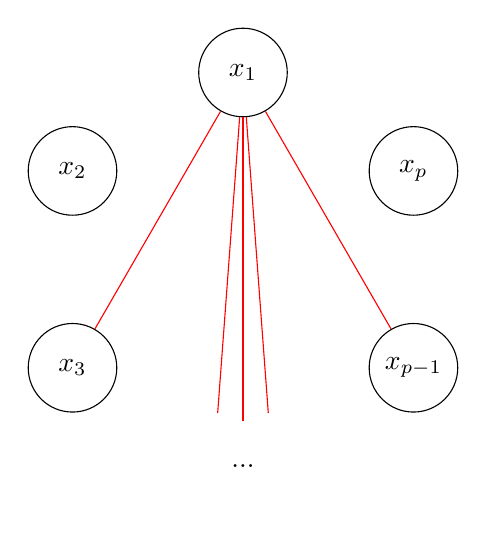
\begin{tikzpicture}[
        point/.style={circle,draw,minimum size=#1},
        point/.default=0pt
    ]
        \node[point=3.2em] (1) at (90:2.5) {$x_1$};
        \node[point=3.2em] (2) at (150:2.5) {$x_2$};
        \node[point=3.2em] (3) at (210:2.5) {$x_3$};
        \node[point=3.2em, draw=none] (dots) at (270:2.5) {...};
        \node[point=3.2em] (pm1) at (330:2.5) {$x_{p-1}$};
        \node[point=3.2em] (p) at (30:2.5) {$x_p$};


        \centerarc[](0,0)(105:135:2.5)
        \centerarc[](0,0)(165:195:2.5)
        \centerarc[](0,0)(225:255:2.5)
        \centerarc[](0,0)(285:314.5:2.5)
        \centerarc[](0,0)(345.5:375:2.5)
        \centerarc[](0,0)(45:75:2.5)

        \draw (1) edge[red] (3);
        \draw (1) edge[red] (dots);
        \draw (1) edge[red] (pm1);
        \draw (1) edge[red] (260:1.85);
        \draw (1) edge[red] (280:1.85);
        
    \end{tikzpicture}
    \caption{The graph $\G = ([p], E)$ formed from the black edges in the above figure is the cycle of length $p$. If $E^+$ is formed by adding the red edges in the figure to $E$, $\G^+ = ([p], E^+)$ forms a chordal cover of $\G$.}
    \label{fig-pcycle}
\end{figure}